\documentclass{article}
\usepackage[a4paper, left=2.5cm, right=2.5cm, top=3cm,bottom=3cm]{geometry}
\usepackage[T1]{fontenc}
\usepackage[utf8]{inputenc}
% \usepackage{todonotes}
% \presetkeys{todonotes}{inline}{}

\usepackage[square, numbers, comma, sort&compress]{natbib}
\renewcommand\refname{References} % Adding title to referece section

\usepackage{xr-hyper} % For cross-referencing between the main article and supporting information
\usepackage[hidelinks]{hyperref}
\usepackage{stackengine} %Stacking symbols
\usepackage[version=4]{mhchem} %chemical equations

\usepackage{siunitx} %get SI units
\DeclareSIUnit{\atm}{atm}
\DeclareSIUnit{\angstrom}{\AA}
\DeclareSIUnit\bar{bar}

\renewcommand{\thefootnote}{\roman{footnote}} % Footnotes using roman numerals

\usepackage{float} %stuff that floats around
% \usepackage{dblfloatfix}    % To enable figure* floats at the bottom of page (figure must be declared before the page on which it should appear)
\usepackage{multirow}
\usepackage{booktabs}  %tables and stuff
\usepackage{tabularx}
\newcolumntype{Y}{>{\centering\arraybackslash}X} % To make tabularx spread the content across the column
\AtBeginDocument{% workaround for \toprule, \midrule and \bottomrule for revtex documentclass
  \heavyrulewidth=.08em
  \lightrulewidth=.05em
  \cmidrulewidth=.03em
  \belowrulesep=.65ex
  \belowbottomsep=0pt
  \aboverulesep=.4ex
  \abovetopsep=0pt
  \cmidrulesep=\doublerulesep
  \cmidrulekern=.5em
  \defaultaddspace=.5em
}


\usepackage{graphicx} %extra options when inputting figures
\usepackage[caption=false]{subfig} %subfigures
\usepackage{afterpage}

\usepackage{enumitem} % for listing stuff (bulletpoints and so on)
\usepackage{setspace} %if you want to change linespacing
\usepackage[parfill]{parskip} %spacing between paragraphs

\usepackage{amsmath, amssymb}
\usepackage{MnSymbol}
\usepackage{mathrsfs} % Nice, curly caligraphic with \mathscr
\usepackage{textgreek}
%Putting self-defined commands here

\renewcommand{\Vec}[1]{\boldsymbol{\mathrm{#1}}} % pretty vectors
\renewcommand{\vec}[1]{\Vec{#1}}
\newcommand{\Mat}[1]{\underline{\pmb{#1}}} % Matrices

% Common symbols
% Fluxes
\newcommand{\bvec}[1]{\Bar{\Vec{#1}}}
\newcommand{\flux}[2]{\Vec{J}_{#1}^{(#2)}}
\newcommand{\mflux}{\Vec{J}^{(n,m)}}
\newcommand{\qflux}{\Vec{J}_q}

% Thermo
% Vectors
\newcommand{\vx}{\vec{x}}
\newcommand{\vn}{\vec{n}}

\newcommand{\Lmm}{L_{\mu \mu}}
\newcommand{\Lmq}{L_{\mu q}}
\newcommand{\Lqm}{L_{q \mu}}
\newcommand{\Lqq}{L_{qq}}

\newcommand{\ST}{S_{T,1}}
\newcommand{\Kr}{K_{\rho}}
\newcommand{\Arho}{A_{\rho}}
\newcommand{\Brho}{B_{\rho}}

\newcommand{\Ta}{T^{\alpha}}
\newcommand{\Tb}{T^{\beta}}
\newcommand{\Va}{V^{\alpha}}
\newcommand{\Vb}{V^{\beta}}
\newcommand{\na}{n^{\alpha}}
\newcommand{\nb}{n^{\beta}}
\newcommand{\xa}{x^{\alpha}}
\newcommand{\xb}{x^{\beta}}
\newcommand{\vna}{\vn^{\alpha}}
\newcommand{\vnb}{\vn^{\beta}}
\newcommand{\vxa}{\vx^{\alpha}}
\newcommand{\vxb}{\vx^{\beta}}


% Kinetic gas theory
\newcommand{\vr}{\vec{r}}
\newcommand{\vu}{\vec{u}}
\newcommand{\bvu}{\Bar{\vec{u}}}
\newcommand{\cvel}[1]{\bvec{u}_{#1}}
\newcommand{\vU}{\vec{U}}
\newcommand{\cVel}{\bvec{U}}
\newcommand{\sD}{\mathscr{D}}
\newcommand{\sU}{\mathscr{U}}
\newcommand{\vsU}{\pmb{\mathscr{U}}}
\newcommand{\vA}{\vec{\Lambda}}
\newcommand{\tvA}{\Tilde{\vA}}
\newcommand{\vD}{\vec{D}}
\newcommand{\vd}{\vec{d}}
\newcommand{\mB}{\Mat{B}}
\newcommand{\va}{\vec{a}}
\newcommand{\sg}{\mathcal{g}}
\renewcommand{\d}{\mathrm{d}}
\newcommand{\rdf}{\Tilde{\chi}}

% Differentials
\renewcommand{\d}{\mathrm{d}}
\newcommand{\dT}{\d T}
\newcommand{\dV}{\d V}
\newcommand{\drho}{\d \rho}
\newcommand{\dr}{\d r}
\newcommand{\dn}{\d n}
\newcommand{\dx}{\d x}
\newcommand{\dA}{\d A}
\newcommand{\dmu}{\d\mu}

% Finite differences
\newcommand{\Dn}{\Delta n}
\newcommand{\Dx}{\Delta x}
\newcommand{\DT}{\Delta T}

\newcommand{\symbline}[3]{$ #1 $ & #2 & \si{#3} \\} % quick symbol table: \symbline{symbol}{description}{unit}
\newcommand{\abrline}[2]{#1 & #2 \\} % Abbreviation & Description
\newcommand{\subline}[2]{$#1$ & #2} % Subscript & Description
%%%%%%%%%%%%%%%%%%%%%%%%%%%%%%%%%%%%%%%%%%%%%%%%%%%%%%%%%%%%%%%%%%%%%%%%%%%%%%%%%%%%%%%%%%%%%%%%%%%%%%%%%%%%
%       quick maffs       %
\newcommand{\del}{\partial} 
\newcommand{\pfrac}[2]{\left(\frac{#1}{#2}\right)} %fraction with parentheses around
\newcommand{\pder}[2]{\frac{\del #1}{\del #2}} %partial derivative of x with respect to y as \pder{x}{y}
\newcommand{\ppder}[2]{\left(\pder{#1}{#2}\right)} %\pder{}{} but with parentheses
\newcommand{\der}[2]{\pfrac{\d #1}{\d #2}}
\newcommand{\lrp}{\left(}
\newcommand{\rrp}{\right)}
\newcommand{\lsp}{\left[}
\newcommand{\rsp}{\right]}
\newcommand{\lcp}{\left\{}
\newcommand{\rcp}{\right\}}
\newcommand{\DeltaAB}{\underset{\alpha,\beta}{\Delta}}
\newcommand{\DeltaIG}{\underset{ig}{\Delta}}
\newcommand{\DeltaHS}{\underset{HS}{\Delta}}
\newcommand{\stackmax}[1]{\stackanchor{$\max$}{\tiny{$#1$}}}

\newcommand{\spder}[3]{
  \ifthenelse{\equal{\detokenize{#2}}{\detokenize{#3}}}
    {\left(\frac{\del^2 #1}{\del #2^2}\right)}
    {\left(\frac{\del^2 #1}{\del #2 \del #3}\right)}%
}

\newcommand{\abs}[1]{\left|#1\right|}
\newcommand{\mathsec}[1]{\texorpdfstring{#1}{TEXT}}

\title{Documentation for multicomponent solutions}
\author{Vegard Gjeldvik Jervell}

\begin{document}

\maketitle

\tableofcontents

\section{Introduction}

The starting point for developing a kinetic model for multicomponent, high density mixtures is the same as that for the binary, single component case, with a minor modification. The Boltzmann equations for an $N$ component mixture may be written as

\begin{equation}
    \lsp \pder{}{t} + \vu_i \cdot \nabla + \pfrac{\Vec{F}_i}{m_i} \cdot \pder{}{\vu_i} \rsp f_i = \sum_j J_{ij}(f_i f_j), \hspace{.5cm} i = \{1, 2, ..., N\}
    \label{eq:boltzmann_multi}
\end{equation}

where $t$ is the time, $\vu_i$ is the velocity, $\Vec{F}_i$ is the sum of external forces, $m_i$ is the mass and $f_i$ is the velocity distribution function (vdf.) of species $i$. $J_{ij}$ is the streaming operator which becomes
\begin{equation}
    J_{ij}(f_i f_j) \equiv \int \int \int \chi_{ij}(\Vec{r}, \Vec{r} + \sigma_{ij}\hat{k}) f_i'(\Vec{r})f_j'(\Vec{r} + \sigma_{ij}\hat{k}) - \chi_{ij}(\Vec{r}, \Vec{r} - \sigma_{ij} \hat{k})f_i(\Vec{r})f_j(\Vec{r} - \sigma_{ij}\hat{k}) b\d b \d \epsilon \d \vu_j
    \label{eq:streaming_op}
\end{equation}

where $\hat{k}$ is the unit vector connecting the two particles, $b$ is the impact parameter and $\epsilon$ is the angular coordinate in the plane of $b$. The prime in $f_i'$ denotes functions of the post-collision velocities. In the same manner as for low-density mixtures, the streaming operator describes the rate of change in the vdf. of species $i$ due to collisions with species $j$. 

The modification when comparing to the low-density streaming operator is the introduction of the factor $\chi_{ij}$, the pair distribution function of the particles, which modifies the probability of finding particles $i$ and $j$ at positions $\Vec{r}_i$ and $\Vec{r}_j$. Furthermore, the vdf. of particle $j$ in the integral of Equation \eqref{eq:streaming_op} is evaluated at $\Vec{r} \pm \sigma_{ij} \hat{k}$ rather than at $\Vec{r}$. Here, $\sigma_{ij}$ is taken to be the distance between the centre of mass of the particles ''at contact''. For hard spheres, this definition is unproblematic but for particles interacting with some realistic potential the definition of being ''at contact'' is slightly less clear. For now, $\sigma_{ij}$ may be regarded as a parameter in the range of the molecular sizes, that is independent of particle velocity and position.

Following the Enskog solution method,\cite{cohen_1} de Haro et al. find that a first approximation to the vdf. may be written as
\begin{equation}
    f_i^{(1)} = f_i^{(0)}\lsp 1 + \Phi_i \rsp
\end{equation}

where 

\begin{equation}
    f_i^{(0)} = n_i \pfrac{m_i}{2 \pi k_B T}^{\frac{3}{2}} \exp \lsp - \sU_i^2 \rsp
    \label{eq:eq_vdf}
\end{equation}

is the Maxwell distribution function, with the peculiar velocity $\vU_i \equiv \vu_i - \vu^m$ defined relative to the \textit{centre of mass} velocity $\vu^m$ and the dimensionless peculiar velocity defined as $\sU_i^2 \equiv \frac{m_i}{2 k_B T}U_i$. $n_i$ is used to denote the particle density of species $i$.

Equivalently to the low-density case, $f_i^{(0)}$ satisfies the conservation equations of mass, energy and momentum exactly. That is,
\begin{equation}
    \begin{split}
        \int f_i^{(0)} \d \vu_i &= n_i, \hspace{.25cm} \forall \hspace{.25cm} i\\
        \sum_i \int f_i^{(0)} m_i \vu_i \d \vu_i &= \rho \vu^m \\
        \sum_i \int f_i^{(0)} \frac{m_i}{2} \vU_i ^2 \d \vu_i &= \frac{3}{2} n k_B T
    \end{split}
\end{equation}

where $\rho$ denotes the mass density of the mixture. Thus, for all $r > 0$ we can require that
\begin{equation}
    \begin{split}
        \int f_i^{(r)} \d \vu_i &= 0, \hspace{.25cm} \forall \hspace{.25cm} i\\
        \sum_i \int f_i^{(r)} m_i \vu_i \d \vu_i &= 0 \\
        \sum_i \int f_i^{(r)} \frac{m_i}{2} \vU_i ^2 \d \vu_i &= 0.
    \end{split}
\end{equation}

The equation of conservation of momentum is obtained by multiplying Equation \eqref{eq:boltzmann_multi} by $m_i \vu_i$. Reordering this equation and inserting for $f_i^{(0)}$, one can identify the hydrostatic pressure as

\begin{equation}
    p = p^k + p^\phi, \hspace{.5cm} p^k = n k_B T, \hspace{.5cm} p^\phi = \frac{2 \pi}{3} n^2 k_B T \sum_i \sum_j x_i x_j \sigma_{ij}^3 \chi_{ij}
\end{equation}

where $x_i$ denotes the mole fraction of species $i$.

In determining the first order approximation to the vdf. it is found that $\Phi_i$ is of the form
\begin{equation}
    \Phi_i = - \frac{1}{n} \vA_i \nabla \ln T - \frac{1}{n} \mB_i : \nabla \vu^m + \frac{1}{n} H_i \nabla \cdot \vu^m - \frac{1}{n} \sum_j \vD_i^{(j)} \vd_j'
\end{equation}

where $\vd_j'$ is defined by

\begin{equation}
    \vd_i = \sum_{j \neq i} \omega_j \vd_i' - \omega_i \vd_j'
\end{equation}

with $\omega_i$ denoting the weight fraction of species $i$ and
\begin{equation}
    \vd_i = - \frac{\rho_i}{\rho n k_B T} \lsp \nabla p + \sum_j \rho_j \lrp \frac{\Vec{F}_i}{m_i} - \frac{\Vec{F}_j}{m_j}\rrp \rsp + \sum_j x_i \lrp \delta_{i,j} + \frac{4 \pi}{3} n_j M_{ij} \sigma_{ij}^3 \chi_{ij}\rrp \nabla \ln T + \frac{x_i}{k_B T} \nabla_T \mu_j
    \label{eq:diffusion_driving_force}
\end{equation}

where $\delta_{i,j}$ is the Kronecker delta and $M_{ij} = \frac{m_i}{m_i + m_j}$. The final term, the gradient in chemical potential at constant temperature may be rewritten as

\begin{equation}
    \frac{x_i}{k_B T} \nabla_T \mu_i = \frac{x_i}{k_B T} \sum_j \ppder{\mu_i}{n_j}_{T,n_{k \neq j}} \nabla n_j
\end{equation}

yielding
\begin{equation}
    \vd_i = - \frac{\rho_i}{\rho n k_B T} \lsp \nabla p + \sum_j \rho_j \lrp \frac{\Vec{F}_i}{m_i} - \frac{\Vec{F}_j}{m_j}\rrp \rsp + \sum_j x_i \lrp \delta_{i,j} + \frac{4 \pi}{3} n_j M_{ij} \sigma_{ij}^3
    \chi_{ij}\rrp \nabla \ln T + \frac{1}{n} E_{ij} \nabla n_j
    \label{eq:diffusion_driving_force2}
\end{equation}

where one should recall that $n_i$ denotes the particle \textit{density} of component $i$.

The response functions $\vA_i$, $\mB_i$, $H_i$ and $\vD_i^{(j)}$ are related to the thermal conductivity, shear viscosity, bulk viscosity and diffusion coefficient of the mixture. In the same manner as for a dilute mixture, one may determine the transport coefficients by writing the response functions as polynomial expansions in the Sonine polynomials, and requiring that these expansions obey the constrains posed by the summational invariants.

In the following sections the resulting equations for the transport coefficients, and their relation to the fluxes will be given. In the case of diffusion, the matter of how the diffusion coefficient should be defined will be addressed.

\section{Diffusion Coefficients}\label{sec:diffusion}

When defining the diffusion coefficients we must make a set of choices:
\begin{itemize}
    \item What frame of reference do the coefficients apply to?
    \item What basis are the fluxes measured in?
    \item What forces are our driving forces?
    \item Are we using an independent or dependent set of driving forces?
    \item If we are using an independent set: What is the dependent driving force?
\end{itemize}

In this memo, the notation $J_i^{(x, f)}$ is used to denote a flux on the $x$ basis, in the $f$ frame of reference, such that a molar flux in the mole-centre frame of reference is denoted $J_i^{(n, n)}$, and the corresponding mass flux is $J_i^{(m, n)} ) = m_i J_i^{(n, n)}$, where $m_i$ is the molar mass of species $i$. Diffusion coefficients are denoted $D_{ij}^{(f,l)}$, where the indices indicate 

\begin{itemize}
    \item $i$ : The flux the diffusion coefficient applies to.
    \item $j$ : The force the diffusion coefficient applies to.
    \item $f$ : The frame of reference the diffusion coefficient applies to.
    \item $l$ : The index of the dependent force. The index $l$ is omitted for diffusion coefficients defined using a dependent set of forces.
\end{itemize}

This indexing may at first seem excessive, but it is required in order to accurately differentiate between the different definitions discussed here. Using this notation, we can write Ficks' law on a molar basis in the centre of moles (CoN) frame of reference (FoR) for an arbitrary multicomponent mixture as
\begin{equation}
    J_i^{(n,n)} = - \sum_{j \neq l} D_{ij}^{(n,l)} \nabla c_j
\end{equation}
where we have used the molar concentrations as driving forces, and chosen to use an independent set of driving forces, as the dependent gradient $\nabla c_l$ is given by
\begin{equation}
    \nabla c_l = - \sum_{j \neq l} \nabla c_j.
\end{equation}

For a binary mixture, taking $l = 2$, this reduces to
\begin{equation}
    \begin{split}
        J_1^{(n, n)} = - D_{11}^{(n, 2)} \nabla c_1, &\quad J_2^{(n, n)} = - D_{21}^{(n, 2)} \nabla c_1, \\
        J_1^{(n, n)} = - J_2^{(n, n)} \quad &\iff \quad D_{11}^{(n, 2)} = - D_{21}^{(n, 2)},
    \end{split}
\end{equation}
a commonly known formulation of Ficks' law in binary mixtures.

To most easily expand our formulation of Ficks' law from binary to multicomponent mixtures, and to facilitate keeping track of indices, the KineticGas always\footnote{See note on the option \code{use\_binary=True}.} returns an $N \times N$ diffusion matrix, defined through
\begin{equation}
    \begin{pmatrix}J_1 \\ J_2 \\ \vdots \\ J_N \end{pmatrix}^{(n, f)} = -
    \begin{bmatrix}
    D_{11} & D_{12} & \hdots & D_{1N} \\
    D_{21} & D_{22} & \hdots & D_{2N} \\
    \vdots & \vdots & \ddots & \vdots \\
    D_{N1} & D_{N2} & \hdots & D_{NN}
    \end{bmatrix}^{(f, l)}
    \begin{pmatrix}\nabla c_1 \\ \nabla c_2 \\ \vdots \\ \nabla c_N \end{pmatrix}
    \label{eq:diff_definition}
\end{equation}
where the dependent species, $l$, is selected with the \code{dependent\_idx} option (default is last component, $l = N$). For the described binary case mentioned above (CoN FoR, species 2 as the dependent species), this reduces to
\begin{equation}
    \begin{pmatrix}J_1 \\ J_2\end{pmatrix}^{(n, n)} = -
    \begin{bmatrix}
    D_{11} & 0 \\
    D_{21} & 0 \\
    \end{bmatrix}^{(n, 2)}
    \begin{pmatrix}\nabla c_1 \\ \nabla c_2\end{pmatrix}
\end{equation}

where, as described above, the coefficients fulfill $D_{11}^{(n, 2)} = - D_{21}^{(n, 2)}$. If we select species 1 as the dependent component, the resulting matrix is
\begin{equation}
    \begin{pmatrix}J_1 \\ J_2\end{pmatrix}^{(n, n)} = -
    \begin{bmatrix}
    0 & D_{12} \\
    0 & D_{22} \\
    \end{bmatrix}^{(n, 1)}
    \begin{pmatrix}\nabla c_1 \\ \nabla c_2\end{pmatrix}
\end{equation}
where, because for a binary mixture at isothermal, isobaric conditions, $\nabla c_1 = - \nabla c_2$, and in the CoN FoR, $J_1^{(n, n)} = - J_2^{(n, n)}$, we have $D_{12}^{(n, 1)} = - D_{11}^{(n, 2)}$ and $D_{22}^{(n, 1)} = - D_{12}^{(n, 1)} = D_{11}^{(n, 2)}$. Because the binary system is often of interest, and we only need on diffusion coefficient to describe the system, using the option \code{use\_binary=True} with the \code{interdiffusion} method, will return the diffusion coefficient
\begin{equation}
    D^{(f)} = D_{11}^{(f, 2)} = D_{22}^{(f, 1)} = - D_{12}^{(f, 1)} = - D_{21}^{(f, 2)}
\end{equation}
where $f$ indicates the frame of reference, such that
\begin{equation}
    J_1^{(n, n)} = - D^{(n)} \nabla c_1,
\end{equation}
the common formulation of Ficks' law in the CoN FoR.

\subsection{Dependent driving forces}
When translating between definitions of the diffusion coefficient it may be convenient to have access to diffusion coefficients defined using a \textit{dependent} set of driving forces. These are then computed by selecting the option \code{use\_independent=False}, and are defined through
\begin{equation}
    \begin{pmatrix}J_1 \\ J_2 \\ \vdots \\ J_N \end{pmatrix}^{(n, f)} = -
    \begin{bmatrix}
    D_{11} & D_{12} & \hdots & D_{1N} \\
    D_{21} & D_{22} & \hdots & D_{2N} \\
    \vdots & \vdots & \ddots & \vdots \\
    D_{N1} & D_{N2} & \hdots & D_{NN}
    \end{bmatrix}^{(f)}
    \begin{pmatrix}\nabla c_1 \\ \nabla c_2 \\ \vdots \\ \nabla c_N \end{pmatrix}
\end{equation}
and in the binary case reduce to
\begin{equation}
    \begin{split}
        J_1^{(n, f)} &= - D_{11}^{(f)} \nabla c_1 - D_{12}^{(f)} \nabla c_2 \\
        J_2^{(n, f)} &= - D_{21}^{(f)} \nabla c_1 - D_{22}^{(f)} \nabla c_2.
    \end{split}
\end{equation}
Note that this diffusion matrix is not unique, and not invertible. It is primarily of interest because it gives easy access to the coefficients given in Eq. (19) of Ref. \cite{retmie}. For practical calculations it is recommended to always use an independent set of driving forces.

\subsection{Frames of Reference}

In the centre of moles (CoN, default) frame of reference (FoR), the molar fluxes are subject to the constraint
\begin{equation}
    \sum_i J_i^{(n, n)} = 0.
\end{equation}
in e.g. CFD calculations, we are typically more interested in fluxes in the centre of mass (CoM, barycentric) FoR. These are subject to the constraint
\begin{equation}
    \sum_i J_i^{(m, m)} = \sum_i m_i J_i^{(n, m)} = 0.
\end{equation}
We compute diffusion coefficients that apply in the CoM FoR by using the option \code{frame\_of\_reference='CoM'} with the \code{interdiffusion} method, which returns the matrix of diffusion coefficients corresponding to the equation
\begin{equation}
    \begin{pmatrix}J_1 \\ J_2 \\ \vdots \\ J_N \end{pmatrix}^{(n, m)} = -
    \begin{bmatrix}
    D_{11} & D_{12} & \hdots & D_{1N} \\
    D_{21} & D_{22} & \hdots & D_{2N} \\
    \vdots & \vdots & \ddots & \vdots \\
    D_{N1} & D_{N2} & \hdots & D_{NN}
    \end{bmatrix}^{(m, l)}
    \begin{pmatrix}\nabla c_1 \\ \nabla c_2 \\ \vdots \\ \nabla c_N \end{pmatrix}
\end{equation}
where, again, $l$ indicates the dependent component (default is last component), and $D_{il} = 0$ for all $i$. This matrix is related to the diffusion matrix in the CoN FoR by the transformation matrix given in the supporting material to Ref. \cite{retmie}.

For all frames of reference (Exception: See section on Ortiz de Zárate.) the definition used for the diffusion coefficients returned by the KineticGas package is that in Eq. \eqref{eq:diff_definition}, that is:
\begin{itemize}
    \item The fluxes are on a \textit{molar basis}.
    \item The driving forces are the \textit{molar concentration gradients}.
\end{itemize}


\section{Thermal diffusion}

This section shows how the thermal diffusion coefficients relate to those in a binary system in the binary limit. The section also gives some insight into different definitions of the thermal diffusion coefficient, with the aim of showing that the definition is not arbitrary if one wishes to relate the ternary coefficients to the respective binary coefficients.

\subsection{Notation}

For fluxes the superscript $(i, j)$ is used, where $i$ is the basis ($m$ for mass-based, $n$ for mole based) and $j$ is the frame of reference. Thermal diffusion coefficients are denoted $D_{T, i}$, the superscript $(z)$ denotes thermal diffusion coefficients as defined by Ortiz de Zárate \cite{ortiz2019definition}, while superscripts $(m)$ and $(n)$ denote the independent thermal diffusion coefficients in the centre of mass, and centre of moles FoR, as defined in ref. \cite{retmie}. 

Similarly, diffusion matrices are superscripted with $(x)$ and $(w)$ to denote those defined by Ortiz de Zárate using the same notation, while superscripts $(m)$ and $(n)$ are used for the independent diffusion matrices in the CoM and CoN FoR as defined in ref. \cite{retmie}.

The notation $D_{T,i}^{(z,tj)}$ denotes the thermal diffusion coefficient of species $i$ in a ternary mixture with species $j$ taken to be the dependent species, as defined in ref. \cite{ortiz2019definition} while $D_{T,i}^{(z,bj)}$ denotes the thermal diffusion coefficient of species $i$ in a binary mixture, with species $j$ taken to be the dependent species.

\subsection{Definitions of the thermal diffusion coefficient}

The default definition of the thermal diffusion coefficient in a multicomponent mixture in the KineticGas package is

\begin{equation}
    J_i^{(n,m)} = D_{T,i}^{(m)} \nabla \ln T - \sum_{j \neq \ell} D_{ij}^{(m)} \nabla c_j
\end{equation}

where the superscript $(n, m)$ indicates that the flux is on a molar basis in the centre of mass (CoM) frame of reference (FoR), and the superscripts $(m)$ indicate that the coefficients apply to the CoM FoR. Component $\ell$ is the dependent component, which defaults to the last component in the mixture. For later convenience, we rewrite this for a ternary system as

\begin{equation}
    \begin{split}
        \begin{pmatrix}J_1^{(n,m)} \\ J_1^{(n,m)} \end{pmatrix} &= - \Mat{D}^{(m)} \begin{pmatrix} \nabla c_1 \\ \nabla c_1 \end{pmatrix} + \begin{pmatrix} D_{T,1}^{(m)} \\ D_{T,2}^{(m)} \end{pmatrix} \nabla \ln T\\
        \Vec{J}^{(n, m)} &= - \Mat{D}^{(m)} \nabla \Vec{c} + \Vec{D}_T^{(m)} \nabla \ln T
    \end{split}
    \label{eq:Dtm_def}
\end{equation}

In the centre of moles frame of reference, the diffusion- and thermal diffusion coefficients are defined by
\begin{equation}
    \begin{split}
        \Vec{J}^{(n, n)} &= - \Mat{D}^{(n)} \nabla \Vec{c} + \Vec{D}_T^{(n)} \nabla \ln T.
    \end{split}
    \label{eq:DTn_def}
\end{equation}
and they are related by
\begin{equation}
    \Mat{D}^{(n)} = \Mat{\Psi}^{n \leftmapsto m} \Mat{D}^{(m)}, \quad \Vec{D}_T^{(n)} = \Mat{\Psi}^{n \leftmapsto m} \Vec{D}_T^{(m)},
\end{equation}
with $\Mat{\Psi}^{n \leftmapsto m}$ being the transformation matrix given in the supporting information of \cite{retmie}, adapted to a $(N_c - 1) \times (N_c - 1)$ matrix, rather than the original $N_c \times N_c$ matrix, by using the linear dependence of the fluxes.

In 2019 Ortiz de Zárate \cite{ortiz2019definition} showed that one can define thermal diffusion coefficients that are equivalent in the centre of mass and centre of moles frames of reference, if one defines them through either

\begin{equation}
    \begin{split}
        \Vec{J}^{(n, n)} &= - c \left( \Mat{D}^{(x)} \nabla \Vec{x} + \Mat{X} \Vec{D}_T^{(z)} \nabla T \right), \quad \text{or}\\
        \Vec{J}^{(m, m)} &= - \rho \left( \Mat{D}^{(w)} \nabla \Vec{w} + \Mat{W} \Vec{D}_T^{(z)} \nabla T \right)
    \end{split}
    \label{eq:zarate_def}
\end{equation}

where the matrices $\Mat{X}$ and $\Mat{W}$ are given by
\begin{equation}
    X_{ij} = \delta_{ij} x_i - x_i x_j, \quad W_{ij} = \delta_{ij} w_i - w_i w_j.
\end{equation}
The superscripts $(x)$ and $(w)$ indicate diffusion matrices that apply in the centre of moles and centre of mass FoR respectively, when using these definitions. The superscript $(z)$ marks the thermal diffusion coefficients as defined by Eq. \eqref{eq:zarate_def}. When using this definition of the thermal diffusion coefficient, Ortiz de Zárate shows that 
\begin{equation}
    \lim_{x_2 \to 0} D_{T,1}^{(z,t3)} = D_{T,1}^{(z,b3)},
\end{equation}
where $D_{T,1}^{(z,t)}$ is the thermal diffusion coefficient of species 1 in a ternary mixture, and $D_{T,1}^{(z,b3)}$ is the thermal diffusion coefficient of species 1 in a binary mixture with species 3, both as defined by Eq. \eqref{eq:zarate_def}.
that is: For a ternary system (1, 2, 3), when the mole fraction of species 2 tends to zero, the thermal diffusion coefficient of species 1 approaches the thermal diffusion coefficient of species 1 in the binary mixture (1, 3). This relation follows from an argument analogous to that in section \ref{sec:diff_indep}.

We can relate the thermal diffusion coefficients $\Vec{D}_T^{(n)}$ to the $\Vec{D}_T^{(z)}$, by rewriting Eq. \eqref{eq:DTn_def} as 
\begin{equation}
    \begin{split}
        \Vec{J}^{(n, n)} &= - \Mat{D}^{(n)} ( c \nabla \Vec{x} + \Vec{x} \nabla c) + \Vec{D}_T^{(n)} \nabla \ln T \\
        &= - \Mat{D}^{(n)} ( c \nabla \Vec{x} - \Vec{x} c \nabla \ln T) + \Vec{D}_T^{(n)} \nabla \ln T \\
        &= - c \Mat{D}^{(n)} \nabla \Vec{x} + \frac{1}{T} \left( \Vec{D}_T^{(n)} + c \Mat{D}^{(n)}\Vec{x}\right) \nabla T
    \end{split}
\end{equation}
such that $\Vec{D}_T^{(z)}$ is given by the solution to
\begin{equation}
    - c \Mat{X} \Vec{D}_T^{(z)} = \frac{1}{T} \left( \Vec{D}_T^{(n)} + c \Mat{D}^{(n)}\Vec{x}\right).
    \label{eq:DTz_DTn_relate}
\end{equation}

By the same manipulation, and noting that we can write $\nabla \vec{x} = \Mat{T}^{x \leftmapsto w} \nabla \Vec{w}$, we can rewrite equation $\eqref{eq:Dtm_def}$ as 
\begin{equation}
    \begin{split}
        \Vec{J}^{(n, m)} &= - \Mat{D}^{(m)} \nabla \Vec{c} + \Vec{D}_T^{(m)} \nabla \ln T \\
        &= - c \Mat{D}^{(m)} \nabla \Vec{x} + \frac{1}{T} \left( \Vec{D}_T^{(m)} + c \Mat{D}^{(m)}\Vec{x}\right) \nabla T \\
        &= - c \Mat{D}^{(m)} \Mat{T}^{x \leftmapsto w} \nabla \Vec{w} + \frac{1}{T} \left( \Vec{D}_T^{(m)} + c \Mat{D}^{(m)}\Vec{x}\right) \nabla T \\
        \Vec{J}^{(m, m)} &= - \diag(\Vec{M}) c \Mat{D}^{(m)} \Mat{T}^{x \leftmapsto w} \nabla \Vec{w} + \frac{1}{T} \diag(\Vec{M}) \left( \Vec{D}_T^{(m)} + c \Mat{D}^{(m)}\Vec{x}\right) \nabla T
    \end{split}
\end{equation}
where $\Vec{M} = (M_1, M_2, ...)^{\top}$ is the vector of molar masses, such that $\Vec{D}_T^{(z)}$ is given by the solution to
\begin{equation}
    - \rho \Mat{W} \Vec{D}_T^{(z)} = \frac{1}{T} \diag(\Vec{M}) \left( \Vec{D}_T^{(m)} + c \Mat{D}^{(m)}\Vec{x}\right).
    \label{eq:DTz_DTm_relate}
\end{equation}

Together, Eqs. \eqref{eq:DTz_DTn_relate} and \eqref{eq:DTz_DTm_relate} allow for a consistency check on the transformation matrices $\Mat{\Psi}^{m \leftmapsto n}$ and $\Mat{\Psi}^{n \leftmapsto m}$, as we should have
\begin{equation}
    \begin{split}
        \frac{1}{c} \Mat{X}^{-1}\left( \Vec{D}_T^{(n)} + c \Mat{D}^{(n)}\Vec{x}\right) &= \frac{1}{\rho} \Mat{W}^{-1} \diag(\Vec{M}) \left( \Vec{D}_T^{(m)} + c \Mat{D}^{(m)}\Vec{x}\right) \\
        &= \frac{1}{\rho} \Mat{W}^{-1} \diag(\Vec{M}) \Mat{\Psi}^{m \leftmapsto n} \left( \Vec{D}_T^{(n)} + c \Mat{D}^{(n)}\Vec{x}\right) \\
        \frac{1}{c} \Mat{X}^{-1} \Mat{\Psi}^{n \leftmapsto m} \left( \Vec{D}_T^{(m)} + c \Mat{D}^{(m)}\Vec{x}\right) &= \frac{1}{\rho} \Mat{W}^{-1} \diag(\Vec{M}) \left( \Vec{D}_T^{(m)} + c \Mat{D}^{(m)}\Vec{x}\right)
    \end{split}
\end{equation}

As a second side-effect of this procedure, we can relate the diffusion matrices, as defined by Eqs. \eqref{eq:zarate_def} to $\Mat{D}^{(m)}$ and $\Mat{D}^{(n)}$ as
\begin{equation}
    \begin{split}
        \Mat{D}^{(x)} &= \Mat{D}^{(n)} \\
        \Mat{D}^{(w)} &= \frac{c}{\rho} \diag(\Vec{M}) \Mat{D}^{(m)} \Mat{T}^{x \leftmapsto w}
    \end{split}
\end{equation}
and remark that Ortiz de Zárate gives the relation
\begin{equation}
    \Mat{W}^{-1} \Mat{D}^{(w)} \Mat{W} = \Mat{X}^{-1} \Mat{D}^{(x)} \Mat{X},
\end{equation}
which can serve as a second consistency check.

All the consistency checks mentioned above have been carried out numerically and been found to pass.

\subsubsection{The binary case}

For convenience, the binary transformations are given explicitly as
\begin{equation}
    \begin{split}
        D_{T,1}^{(z,b3)} &= - \frac{D_{T,1}^{(n, b3)} + c_1 D_{11}^{(n, b3)}}{c_1 (1 - x_1) T} \\
        &= - \frac{D_{T,1}^{(m, b3)} + c_1 D_{11}^{(m, b3)}}{c_1 (1 - w_1) T}
    \end{split}
\end{equation}

\subsection{The binary limit}

With the path to obtaining $\Vec{D}_T^{(z)}$ established, we can now investigate the binary limit of a ternary system. The ternary system investigated consists of species (1, 2, 3) and has the molar composition $\Vec{x}_t = (x_1(1 - x_2), x_2, (1 - x_1)(1 - x_2))$. We are comparing it to a binary system of species (1, 3) with composition $\Vec{x}_b = (x_1, 1 - x_1)$, such that the systems are exactly equivalent when $x_2 = 0$. In both systems we take species 3 to be the dependent species.

The results are shown in Figs. \ref{fig:ternary_DT} and \ref{fig:ternary_DT_large}.

\begin{figure}[htb]
    \centering
    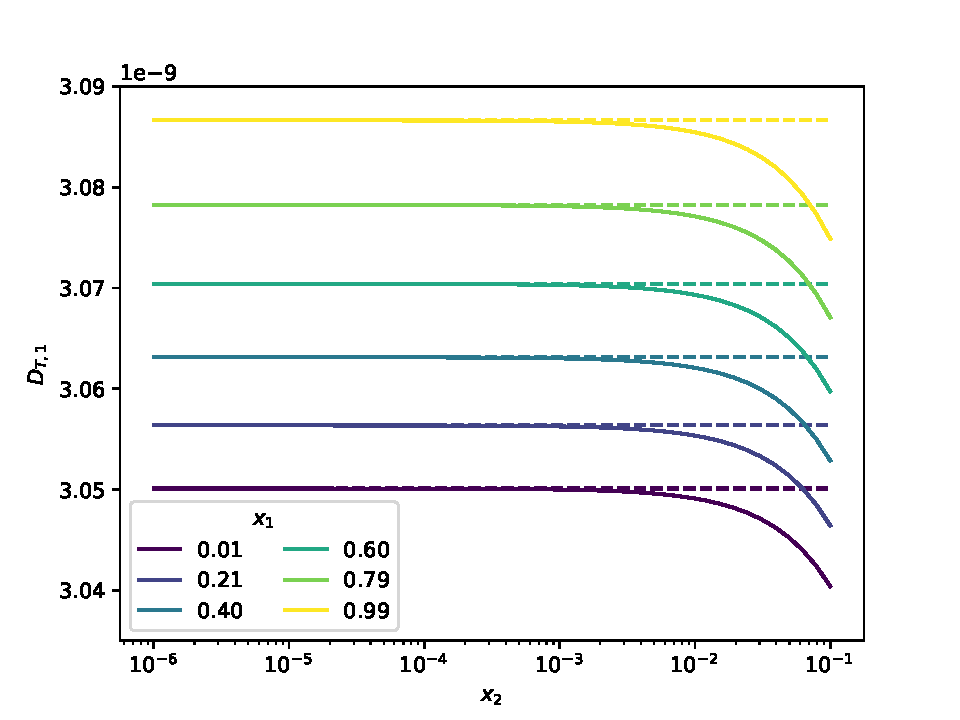
\includegraphics[width=.6\textwidth]{ternary_DT.pdf}
    \caption{The thermal diffusion coefficient $D_{T,1}^{(z, t)}$ in the ternary mixture (1, 2, 3) (solid lines), and the thermal diffusion coefficient $D_{T,1}^{z, b3}$ in the binary mixture (1, 3) (dashed lines), at different mole fractions of species 1 (colors). $x_1$ indicates the mole fraction of species 1 in the binary, i.e. $x_1 = n_1 / (n_1 + n_3)$, such that the composition of the ternary is $\Vec{x}_t = (x_1(1 - x_2), x_2, (1 - x_1)(1 - x_2))$.}
    \label{fig:ternary_DT}
\end{figure}

As seen immediately from Fig. \ref{fig:ternary_DT}, the ternary coefficient (solid lines) approaches the expected binary coefficient as $x_2 \to 0$. Note also the logarithmic scale, and that even at mole fractions of species 2 as small as $x_2 = 10^{-2}$, there is an appreciable difference in $D_{T,1}$ in the ternary compared to the corresponding binary. As seen more clearly in Fig. \ref{fig:ternary_DT_large}, the effect of increasing $x_2$ on $D_{T,1}$ is largest when $x_1$ is large. This could indicate that, contrary to intuition, if one wishes to model a ternary system with $x_1 > x_2 \gg x_3$ as a binary, neglecting the presence of species 3, a better estimate for thermal diffusion is obtained by taking species 2 as the independent species.

Explicitly: For a ternary system consisting of a trace component in air, the best estimate for thermal diffusion appears to be obtained if one models this as a binary mixture of nitrogen with the tracer \textit{taking the tracer to be the independent species}.

\begin{figure}[htb]
    \centering
    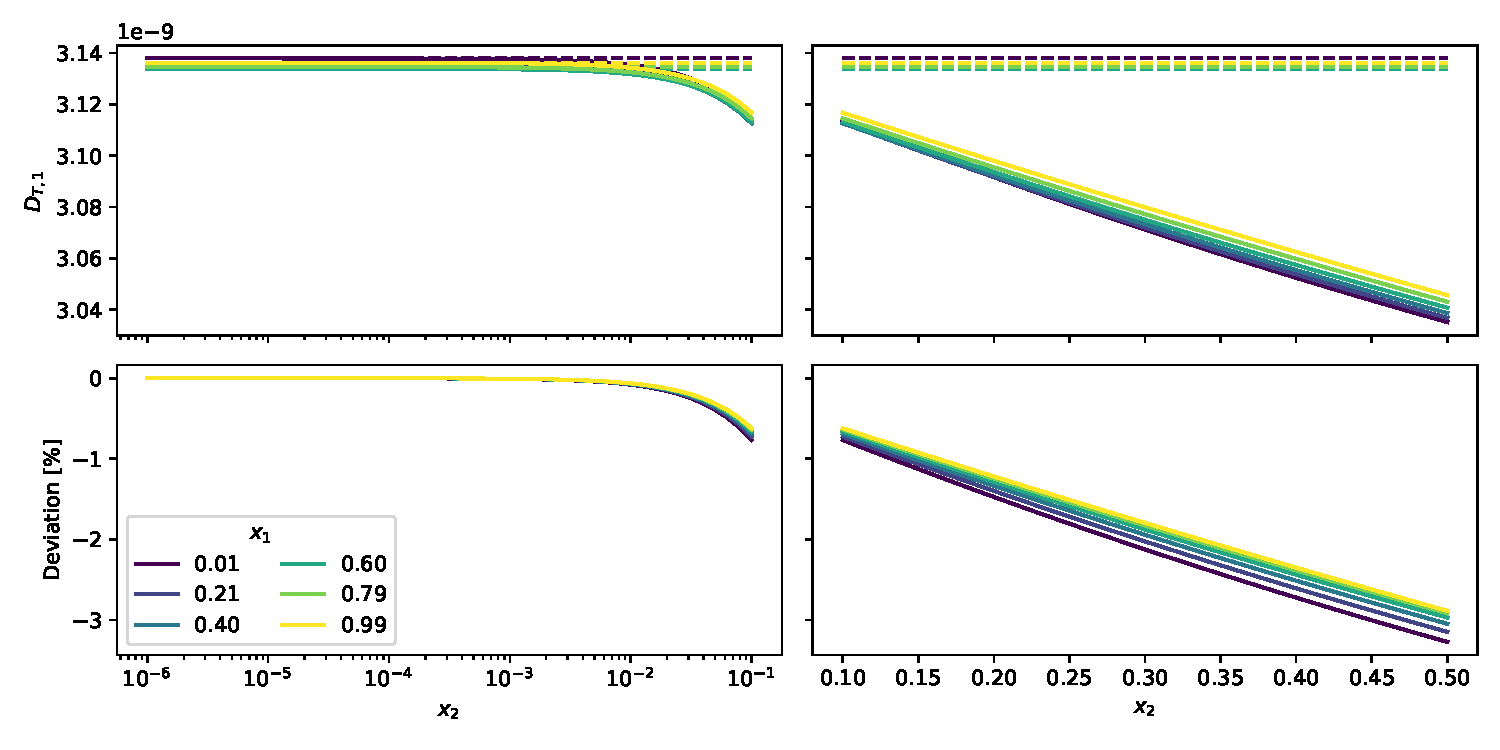
\includegraphics[width=.85\textwidth]{ternary_DT_large.pdf}
    \caption{The same thermal diffusion coefficients as in Fig. \ref{fig:ternary_DT}, with deviations and for a larger composition span.}
    \label{fig:ternary_DT_large}
\end{figure}

\section{Thermal Conductivity}

The heat flux in the centre of mass frame of reference is related to the vdf. as
\begin{equation}
    \qflux = \sum_i \int f_i \frac{m_i}{2}\vU_i^2 d\vu_i
\end{equation}

Having obtained expressions for the thermal- and diffusive response functions, $\vA_i$ and $\vD_i^{(j)}$ in the previous sections this integral may be evaluated to yield

\begin{equation}
    \begin{split}
        \qflux &= - \frac{5 k_B T}{4n} \sum_i K_i x_i \lrp a_i^{(1)} \nabla \ln T - \sum_j d_{i,j}^{(1)} \vd_j\rrp \\
        &\hspace{1cm} - \frac{4 k_B T}{3} \sum_i \sum_j \pfrac{2\pi m_i m_j kB T}{m_i + m_j}^{\frac{1}{2}} \frac{n_i n_j \sigma_{ij}^4 \chi_{ij}}{m_i + m_j} \nabla \ln T\\
        &\hspace{1cm} + k_B T \sum_i \sum_j \frac{2 \pi}{3} n_j \sigma_{ij}^3 (M_{ij} - M_{ji})\chi_{ij}\mflux_i\\
        &\hspace{1cm} + \frac{5 k_B T}{2} \sum_i \lrp 1 + \sum_j\frac{2 \pi}{3} n_i \sigma_{ij}^3\chi_{ij}\rrp \frac{m_i}{m_j} \mflux_i.
    \end{split}
    \label{eq:heat_flux_general}
\end{equation}

In the absence of a mass flux, Fouriers law applies and we have
\begin{equation}
    \qflux = - \lambda \nabla T
    \label{eq:fouriers_law}
\end{equation}

where $\lambda$ is the conductivity. When all mass fluxes vanish in the presence of a temperature gradient, the molar density gradients in $\vd_i$ may be replaced by the thermal diffusion ratios, such that

\begin{equation}
    \begin{split}
        \vd_i &= \sum_j x_i \lrp \delta_{i,j} + b_{ij} - k_{T,i} E_{ji} \rrp  \nabla \ln T, \hspace{1cm} \mflux_k = 0 \hspace{.5cm} \forall \hspace{.5cm} k\\
        &\equiv \sum_j d_j^{th} \nabla \ln T,
    \end{split} 
\end{equation}
where the second equality defines $d_j^{th}$. Furthermore, because all mass fluxes have vanished, these $d_j^{th}$ must satisfy
\begin{equation}
    \sum_j d_{i,j}^{(0)} d_j^{th} = a_i^{(0)} 
\end{equation}

as is seen by setting the left hand side of Equation \eqref{eq:molar_flux_with_temp} to zero. Comparing Equations \eqref{eq:heat_flux_general} and \eqref{eq:fouriers_law} we identify the thermal conductivity as

\begin{equation}
    \begin{split}
        \lambda &= - \frac{5 k_B T}{4n} \sum_i K_i x_i \lrp a_i^{(1)} - \sum_j d_{i,j}^{(1)} d_j^{th}\rrp \\
        &\hspace{1cm} - \frac{4 k_B T}{3} \sum_i \sum_j \pfrac{2\pi m_i m_j k_B T}{m_i + m_j}^{\frac{1}{2}} \frac{n_i n_j \sigma_{ij}^4 \chi_{ij}}{m_i + m_j}
    \end{split}
\end{equation}
\section{Viscosity}
The flux of momentum $\Mat{P}$ is related to the velocity distribution function as 
\begin{equation}
    \Mat{P} = \sum_i \int f_i m_i \vU_i \d \vu_i.
    \label{eq:momentum_flux}
\end{equation}

The hydrodynamic response functions $\Mat{B}_i$ and $H_i$ may be written as the polynomial expansions

\begin{equation}
    B_i = \frac{m_i}{2 k_B T} \sum_{r = 0}^\infty b_i^{(r)} S_{5/2}^{(r)}(\vsU^2), \hspace{1cm} H_i = \sum_{r = 0}^{\infty} h_r^{(0)} S_{1/2}^{(r)}(\vsU^2)
\end{equation}
where $B_i$ is defined by $\Mat{B}_i \equiv B_i\lrp \vU_i \vU_i - \frac{1}{3}U_i^2 \Mat{I}\rrp$. Inserting these expansions into Equation \eqref{eq:momentum_flux}, and applying the conservation law for momentum yields a set of equations for the expansion coefficients as
\begin{equation}
    \sum_{j = 1}^s \sum_{q = 0}^N B_{ij}^{(pq)} b_j^{(q)} = \frac{2}{k_B T}x_i K_i' \delta_{p,0}, \hspace{1cm}
    \begin{cases}
        i = \{1, 2, ..., s\} &\\
        p = \{0, 1, ..., N\} &
    \end{cases}
\end{equation}

where 

\begin{equation}
    \begin{split}
        K_i' &= 1 + \frac{8 \pi n}{15} \sum_j x_j M_{ji} \sigma_{ij}^3 \chi_{ij}\\
        B_{ij}^{(pq)} &= \frac{2}{5 k_B T} \left\{ x_i x_j \lsp S_{5/2}^{(p)}(\vsU_i^2)\overset{\circ}{\vsU_i \vsU_i}, S_{5/2}^{(q)}(\vsU_j^2)\overset{\circ}{\vsU_j \vsU_j} \rsp_{ij}\right. \\
        &\hspace{2cm} \left.+ \delta_{i,j} \sum_k x_i x_k \lsp S_{5/2}^{(p)}(\vsU_i^2)\overset{\circ}{\vsU_i \vsU_i}, S_{5/2}^{(q)}(\vsU_i^2)\overset{\circ}{\vsU_i \vsU_i} \rsp_{ik}\right\}
    \end{split}
\end{equation}

with 
\begin{equation}
    \overset{\circ}{\vsU_i \vsU_i} \equiv \vsU \vsU - \frac{1}{3}\sU^2 \Mat{I}.
\end{equation}

These bracket integrals are exactly the ones identified by Thompson et al. as linear combinations of the collision integrals.\cite{kinetics_viscosity}

\subsection{Determining the expansion coefficients}

\subsection{Flux force relations}

\subsection{Viscosity in terms of the expansion coefficients}

Comparing Equations ... and ... one can identify the shear viscosity as
\begin{equation}
    \eta = \frac{k_B T}{2} \sum_i K_i' x_i b_i^{(0)} + \frac{4}{15} \sqrt{2 \pi k_B T} \sum_i \sum_j \sqrt{\frac{m_i m_j}{m_i + m_j}} n_i n_j \sigma_{ij}^4 \chi_{ij}
\end{equation}
\section{Contact diameters}

The ''contact diameter'', $\sigma_{ij}$ has been mentioned several times thus far, and has been taken to be some distance in the range of the particle sizes. In the case of additive hard spheres, the contact diameter can unambiguously be defined as the distance between the centre of mass of the two particles at contact. However, for Mie particles this definition is not equally straight forward. In this section, various ways of defining the contact diameter, and the inherent underlying assumptions behind the different definitions will be discussed.

Firstly, it is worth mentioning that applying the multicomponent, density corrected solutions proposed by de Haro et al. to Mie fluids implies the assumption that the contact diameters are independent of particle velocities at collision. This assumption is necessary due to the fact that the integral of Equation \eqref{eq:streaming_op} is one over the velocity space. The contact diameters are permitted to be functions of the temperature, and thereby the mean velocities, as well as density and composition but must be constant for all particles in a given state.

One could, in principle, define the contact diameters as some function of the velocities, but this would severely limit the possibility of utilising previously obtained results from the literature. Therefore, such an approach has not been attempted here.

When defining the contact diameters of Mie particles, we note the two roles this distance plays. The first is describing the covolume of the mixture, and the modified probability of finding two particles at contact through the radial distribution function ''at contact''. The second is describing the instantaneous transfer of energy and momentum from one particle to the other when particles collide. This effect manifests itself as the second terms in the expressions for the conductivity and viscosity, which depends on the density, contact diameters and rdf. but not on the polynomial expansion coefficients. Because the contact diameter plays two distinctly different roles, it is not necessarily so that the length one should use in these two roles must be the same.

To evaluate the radial distribution function ''at contact'' a highly convenient choice of the contact diameter is the Mie parameter $\sigma_{ij}$. This allows one to directly apply the expressions proposed by Lafitte et al. for the rdf. at contact.\cite{lafitte2013accurate} This formulation of the rdf. at contact has been shown to give accurate predictions of thermodynamic properties of fluids, and the associated distance is therefore likely to give a good representation of the covolume of the mixture. Therefore, it is believed that using $\sigma_{ij}$ as the contact diameter when computing the rdf. at contact is not only a convenient choice, but also a choice that allows accurate representation of the modified probability of contact between particles due to volume exclusion.

Regarding the second property described by the contact diameter, the instantaneous transfer of energy and momentum at the moment of collision, a distance more directly related to the collision dynamics was chosen. Firstly, note that the equilibrium vdf. given in Equation \eqref{eq:eq_vdf} does not depend on the contact diameters. We regard a colliding pair of particles, and define the contact diameter as the average distance of closest approach ($R$) during collision where the particles repel each other (e.g. collisions where $\theta < \frac{\pi}{2}$). Further, we compute this average for a mixture at equilibrium, when $f_i = f_i^{(0)}$. The contact diameter is then given by

\begin{equation}
    \Bar{R}_{ij} = \int_{0}^{\infty} \int_0^{b'} R_{ij}(g_{ij}, b) \d b \d g_{ij}
    \label{eq:R_defl}
\end{equation}

where $g_{ij}$ is the relative speed of the colliding pair and $b'$ is the solution to the equation

\begin{equation}
    \theta_{ij}(b'; g_{ij}) = 0.
\end{equation}

This integral is somewhat computationally expensive to evaluate, but may be simplified by noting that $R(g_{ij}; b)$ is reasonably symmetric about $g = \Bar{g}$, the average relative speed, as shown in Figure \ref{fig:symmetry_closest_appr}. Due to this symmetry, a good approximation to the integral of Equation \eqref{eq:R_defl} is given by

\begin{equation}
    \Bar{R}_{ij} = \int_0^{\Bar{b}'} R_{ij}(b; \Bar{g}_{ij}) \d b
\end{equation}
with $\Bar{b}'$ given by
\begin{equation}
    \theta_{ij}(\Bar{b}'; \Bar{g}_{ij}) = 0.
\end{equation}

\begin{figure}[htb]
    \centering
    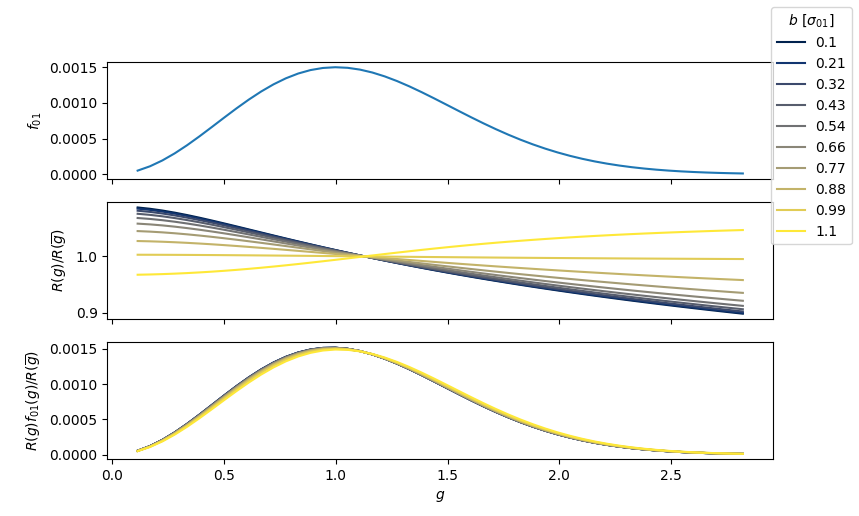
\includegraphics[width=\textwidth]{symmetry_closest_appr}
    \caption{The distance of closest approach as a function of dimensionless relative velocity $g$ and impact parameter $b$ at $T = \SI{500}{\kelvin}$}
    \label{fig:symmetry_closest_appr}
\end{figure}

This integral was evaluated using a six-point Gauss-Legendre quadrature, after investigating the convergence behaviour of the quadrature and finding that this was sufficient to achieve a relative precision of $\approx 10^{-8}$.

\bibliographystyle{ieeetr}
\bibliography{bibliografi}

\end{document}

\section{Conductivity}
To compute the conductivity, we must first find the Sonine polynomial expansion coefficients related to the temperature response function of component $i$, $\Vec{A}_i$, denoted $a_q^{(i)}$. To do this solve the set of equations 
\begin{equation}
    \sum_{j = 1}^s \sum_{q = 0}^{N} \Lambda_{ij}^{pq} a_q^{(j)} = \frac{4}{5k_B}x_i K_i \delta_{p,1}, \hspace{1cm} s = \{1, 2, ..., s\}, p = \{0, 1, ..., N\}
\end{equation}
where $s$ is the number of components, $N$ is the order of the Enskog approximation and $K_i$ is given by
\begin{equation}
    K_i = 1 + \frac{12}{5}\sum_{j = 1}^s \rho b_{ij} M_{ij} M_{ji} g_{ij}
\end{equation}
where $M_{ij} = \frac{m_i}{m_i + m_j}$, $\rho b_{ij} = \frac{2 \pi}{3} n_j \sigma_{ij}^3$ and $g_{ij}$ is the radial distribution function at contact. $\sigma_{ij}$ is taken to be the contact distance of the rdf.

Solve this set of equations by writing it in matrix form as 
\begin{equation}
    \Mat{\Lambda} \Vec{a} = \pmb{\lambda}
\end{equation}
with
\begin{equation}
    \Mat{\Lambda} = \left.\overbrace{
    \begin{bmatrix}
\Lambda_{11}^{00} & \Lambda_{12}^{00} & \hdots & \Lambda_{1s}^{00} & \Lambda_{11}^{01} & \hdots & \hdots & \Lambda_{1s}^{01} & \hdots & \hdots & \Lambda_{1s}^{0N} \\
\Lambda_{21}^{00} & \ddots & & \vdots & \vdots & \ddots & & \vdots & \ddots & & \vdots \\
\vdots & & \ddots & \vdots & \vdots & & \ddots & \vdots & & \ddots & \vdots \\
\Lambda_{s1}^{00} & \Lambda_{s2}^{00} & \hdots & \Lambda_{ss}^{00} & \Lambda_{s1}^{01} & \hdots & \hdots & \Lambda_{ss}^{01} & \hdots & \hdots & \Lambda_{ss}^{0N} \\
\Lambda_{11}^{10} & \Lambda_{12}^{10} & \hdots & \Lambda_{1s}^{10} & \Lambda_{11}^{11} & \hdots & \hdots & \Lambda_{1s}^{11} & \hdots & \hdots & \Lambda_{1s}^{1N} \\
\vdots & \ddots & & \vdots & \vdots & \ddots & & \vdots & \ddots & & \vdots \\
\vdots & & \ddots & \vdots & \vdots & & \ddots & \vdots & & \ddots & \vdots \\
\Lambda_{s1}^{10} & \hdots & \hdots & \Lambda_{ss}^{10} & \Lambda_{s1}^{11} & \hdots & \hdots & \Lambda_{ss}^{11} & \hdots & \hdots & \Lambda_{ss}^{1N} \\
\vdots & \ddots & & \vdots & \vdots & \ddots & & \vdots & \ddots & & \vdots \\
\vdots & & \ddots & \vdots & \vdots & & \ddots & \vdots & & \ddots & \vdots \\
\Lambda_{s1}^{N0} & \hdots & \hdots & \Lambda_{ss}^{N0} & \Lambda_{s1}^{N1} & \hdots & \hdots & \Lambda_{ss}^{N1} & \hdots & \hdots & \Lambda_{ss}^{NN} \\
    \end{bmatrix}
    }^{Ns} \right\} Ns
\end{equation}

which for clarity may be written as an ($N \times N$) block matrix
\begin{equation}
    \Mat{\Lambda} = 
    \begin{bmatrix}
        \Mat{\Lambda}^{(00)} & \Mat{\Lambda}^{(01)} & \hdots & \Mat{\Lambda}^{(0N)} \\
        \Mat{\Lambda}^{(10)} & \ddots             &        & \vdots \\
        \vdots             &                    & \ddots & \vdots \\
        \Mat{\Lambda}^{(N0)} & \hdots & \hdots  & \Mat{\Lambda}^{(NN)}
    \end{bmatrix}
    \label{eq:lambda_block1}
\end{equation}
consisting of ($s \times s$) blocks
\begin{equation}
    \Mat{\Lambda}^{(pq)} = 
    \begin{bmatrix}
        \Lambda_{11}^{pq} & \Lambda_{12}^{pq} & \hdots & \Lambda_{1s}^{pq} \\
        \Lambda_{21}^{pq} & \ddots & & \vdots \\
        \vdots & & \ddots & \vdots \\
        \Lambda_{s1}^{pq} & \hdots & \hdots & \Lambda_{ss}^{pq} 
    \end{bmatrix}.
    \label{eq:lambda_block2}
\end{equation}

The corresponding vectors $\Vec{a}$ and $\Vec{\delta}$ are then

\begin{equation}
    \Vec{a} = 
    \begin{pmatrix}
        a_0^{(1)} \\ a_0^{(2)} \\ \vdots \\ a_0^{(s)} \\ a_1^{(1)} \\ \vdots \\ a_{1}^{(s)} \\ \vdots \\ a_{N}^{(s)}
    \end{pmatrix}
    , \hspace{2cm}
    \pmb{\lambda} = \frac{4}{5k_B}
    \begin{pmatrix}
        0 \\ \vdots \\ \times s \\ \vdots \\ 0 \\ x_1 K_1 \\ x_2 K_2 \\ \vdots \\ x_s K_s \\ 0 \\ \vdots \\ \times (N - 2)s \\ \vdots \\ 0
    \end{pmatrix}.
\end{equation}

The $\Lambda_{ij}^{pq}$ elements are evaluated as
\begin{equation}
    \Lambda_{ij}^{pq} = \frac{8}{75 k_B^2 T} \sqrt{m_1 m_2} \left\{ x_i x_j g_{ij} \left[S_{3/2}^{(p)}(\vsU_i^2)\vsU_i, S_{3/2}^{(q)}(\vsU_j^2)\vsU_j\right]_{ij} + \delta_{i,j} \sum_{\ell = 1}^{s} x_i x_\ell g_{i\ell} \left[S_{3/2}^{(p)}(\vsU_i^2)\vsU_i, S_{3/2}^{(q)}(\vsU_i^2)\vsU_i\right]_{i\ell} \right\}
    \label{eq:lambda_coeffs}
\end{equation}
where $[F_i, G_j]_{ij}$ and $[F_i, G_i]_{ij}$ refer to the bracket integrals to which Thompson, Tipton and Lloyalka have identified summational expressions for and $\delta_{i,j}$ is the Kronecker delta.

The conductivity is given in terms of the expansion coefficients $\Vec{a}_q^{(j)}$ as 
\begin{equation}
    \begin{split}
        \lambda &= \frac{5 k_B}{4} \sum_{i} x_i \left(1 + \frac{12}{5} \sum_{j} \rho b_{ij} M_{ij} M_{ji} g_{ij} \right)\left(a_1^{(i)} - \sum_{k} d_{i,1}^{(k)}d_k^{th}\right) \\
        & \hspace{.5cm} +\frac{5 k_B}{4} \sum_i \sum_j \sqrt{\frac{2\pi m_i m_j k_B T}{m_i + m_j}} \frac{n_i n_j}{m_i + m_j}\sigma_{ij}^{4} g_{ij}
    \end{split}
\end{equation}
where the sums run over the components of the mixture. The expression may be simplified somewhat by inserting for $K_i$ to yield
\begin{equation}
    \begin{split}
        \lambda &= \frac{5 k_B}{4} \sum_{i} x_i K_i \left(a_1^{(i)} - \sum_{k} d_{i,1}^{(k)}d_k^{th}\right) \\
        & \hspace{.5cm} +\frac{5 k_B}{4} \sum_i \sum_j \sqrt{\frac{2\pi m_i m_j k_B T}{m_i + m_j}} \frac{n_i n_j}{m_i + m_j}\sigma_{ij}^{4} g_{ij}.
    \end{split}
\end{equation}
The coefficients $d_k^{th}$ are found by the solving the set of equations 
\begin{equation}
    \sum_{k = 1}^s d_{i,0}^{(k)} d_k^{th} = a_0^{(i)}, \hspace{1cm} i = \{1, 2, ..., s\},
    \label{eq:dth_set}
\end{equation}
with $d_{i,0}^{(k)}$ given by the solution to the diffusion equations \eqref{eq:diffusion_eq_matr}. Written in matrix form, equation \eqref{eq:dth_set} reads
\begin{equation}
    \Mat{D}_{th} \Vec{d}_{th} = \Vec{a}_0
\end{equation}
with 
\begin{equation}
    \Mat{D}_{th} = 
    \begin{bmatrix}
        d_{1, 0}^{(1)} & d_{1, 0}^{(2)} & \hdots & d_{1, 0}^{(s)} \\
        d_{2, 0}^{(1)} & \ddots & & \vdots \\
        \vdots & & \ddots & \vdots \\
        d_{s, 0}^{(1)} & d_{s, 0}^{(2)} & \hdots & d_{s, 0}^{(s)}
    \end{bmatrix}
    , \hspace{1cm}
    \Vec{a_0} = 
    \begin{pmatrix}
        a_0^{(1)} \\ a_0^{(2)} \\ \vdots \\ a_0^{(s)}
    \end{pmatrix}
\end{equation}




